% ------------------------------------------------------------------------------
% TYPO3 CMS 7.6 - What's New - Chapter "In-Depth Changes" (English Version)
%
% @author	Patrick Lobacher <patrick@lobacher.de> and Michael Schams <schams.net>
% @license	Creative Commons BY-NC-SA 3.0
% @link		http://typo3.org/download/release-notes/whats-new/
% @language	English
% ------------------------------------------------------------------------------
% LTXE-CHAPTER-UID:		7229f1b9-b481e9bc-09c46183-a86b6a7e
% LTXE-CHAPTER-NAME:	In-Depth Changes
% ------------------------------------------------------------------------------

\section{In-Depth Changes}
\begin{frame}[fragile]
	\frametitle{In-Depth Changes}

	\begin{center}\huge{Chapter 3:}\end{center}
	\begin{center}\huge{\color{typo3darkgrey}\textbf{In-Depth Changes}}\end{center}

\end{frame}

% ------------------------------------------------------------------------------
% LTXE-SLIDE-START
% LTXE-SLIDE-UID:		f9d6186c-be5505bd-aeab1b8f-46c4a31d
% LTXE-SLIDE-ORIGIN:	159a2d7f-b679989c-30cf1736-6693f827 English
% LTXE-SLIDE-TITLE:		Bootstrap for Install Tool (1)
% ------------------------------------------------------------------------------

\begin{frame}[fragile]
	\frametitle{In-Depth Changes}
	\framesubtitle{Bootstrap for Install Tool (1)}

	\begin{itemize}

		\item The Install Tool is now based on Bootstrap - for the installation part:

			\begin{figure}
				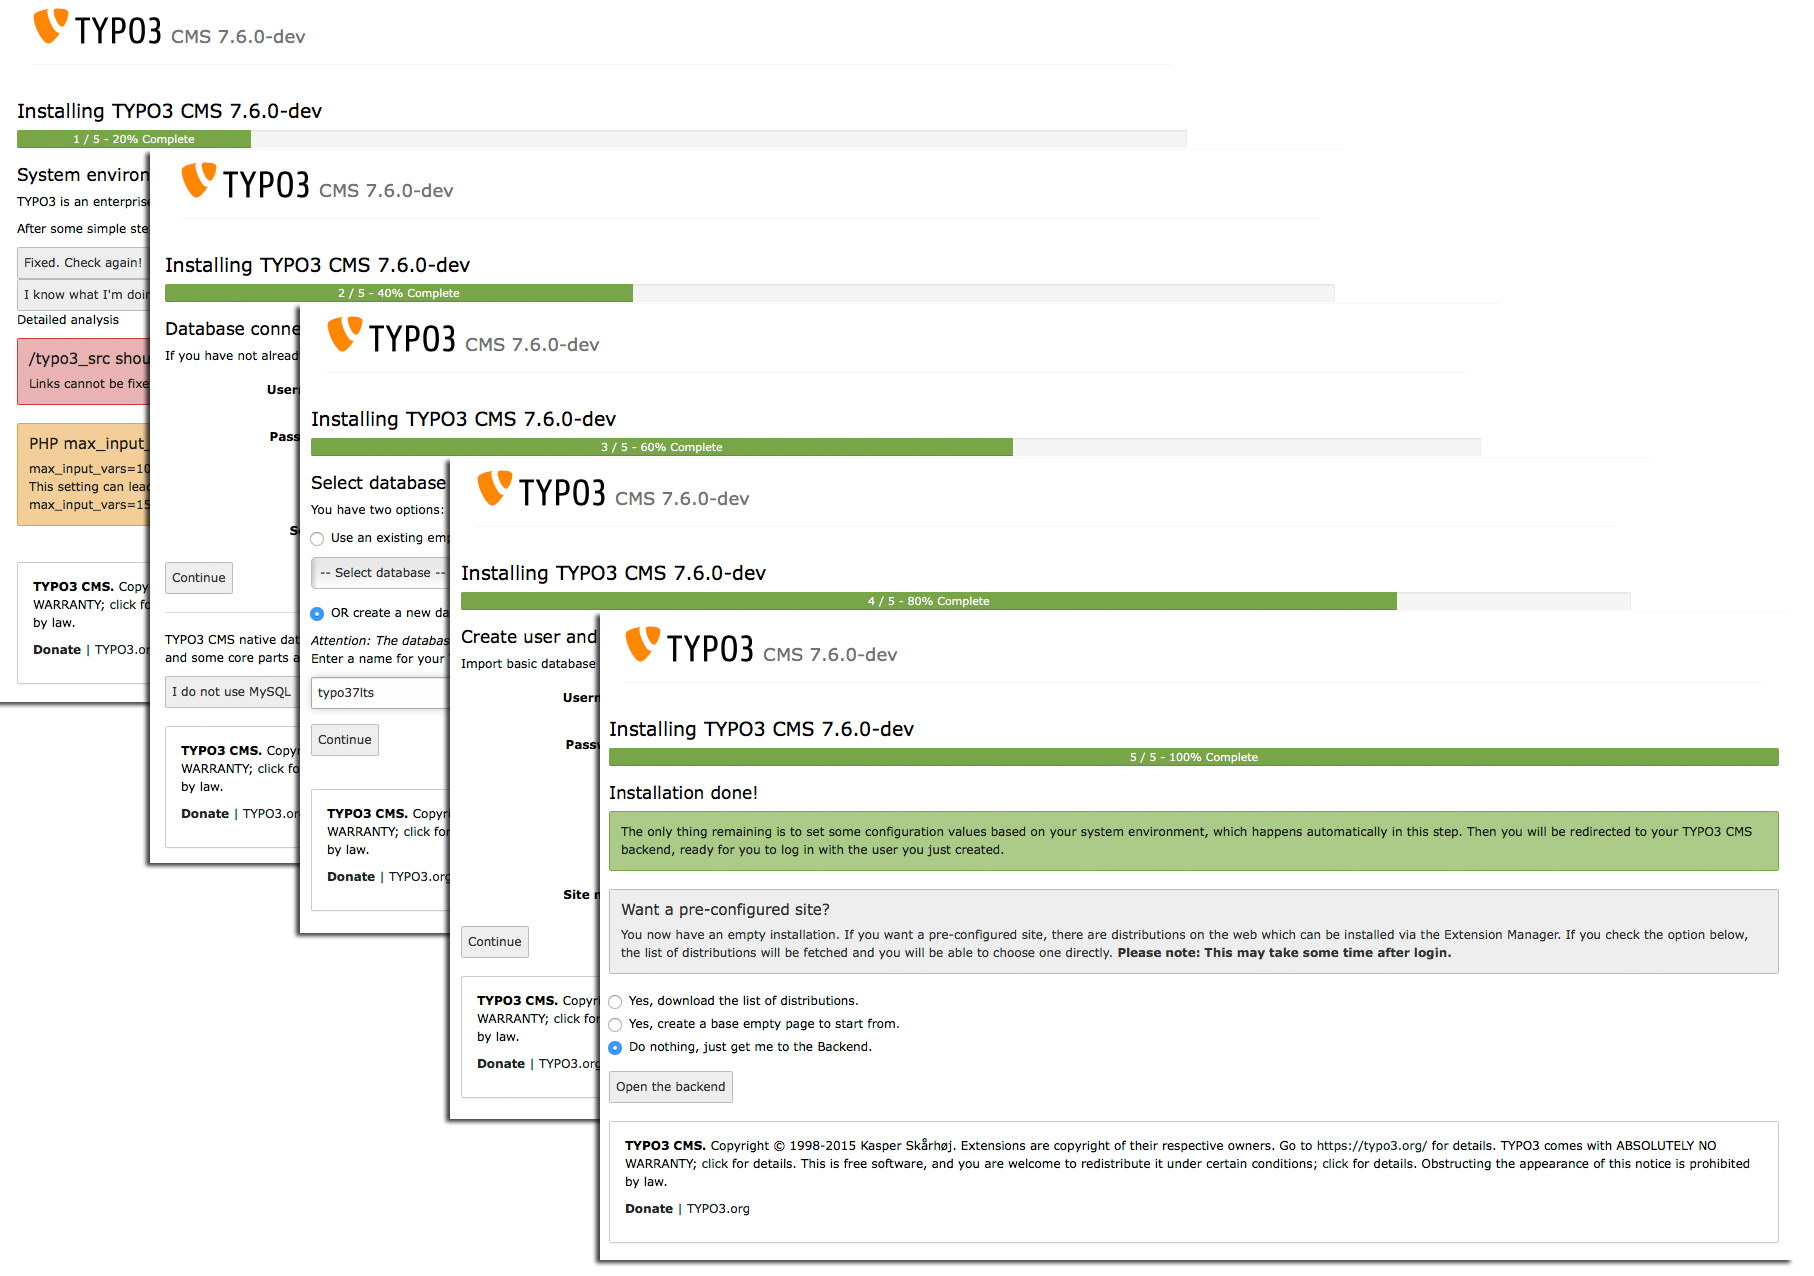
\includegraphics[width=0.7\linewidth]{InDepthChanges/InstallToolBootstrap01.jpg}
			\end{figure}

	\end{itemize}

\end{frame}

% ------------------------------------------------------------------------------
% LTXE-SLIDE-START
% LTXE-SLIDE-UID:		b4b84b2f-b461a032-a7bae892-d6f65392
% LTXE-SLIDE-ORIGIN:	66a71f73-91b6c90e-e548a037-e2d47f94 English
% LTXE-SLIDE-TITLE:		Bootstrap for Install Tool (2)
% ------------------------------------------------------------------------------

\begin{frame}[fragile]
	\frametitle{In-Depth Changes}
	\framesubtitle{Bootstrap for Install Tool (2)}

	\begin{itemize}

		\item The Install Tool is now based on Bootstrap - for the configutation:

			\begin{figure}
				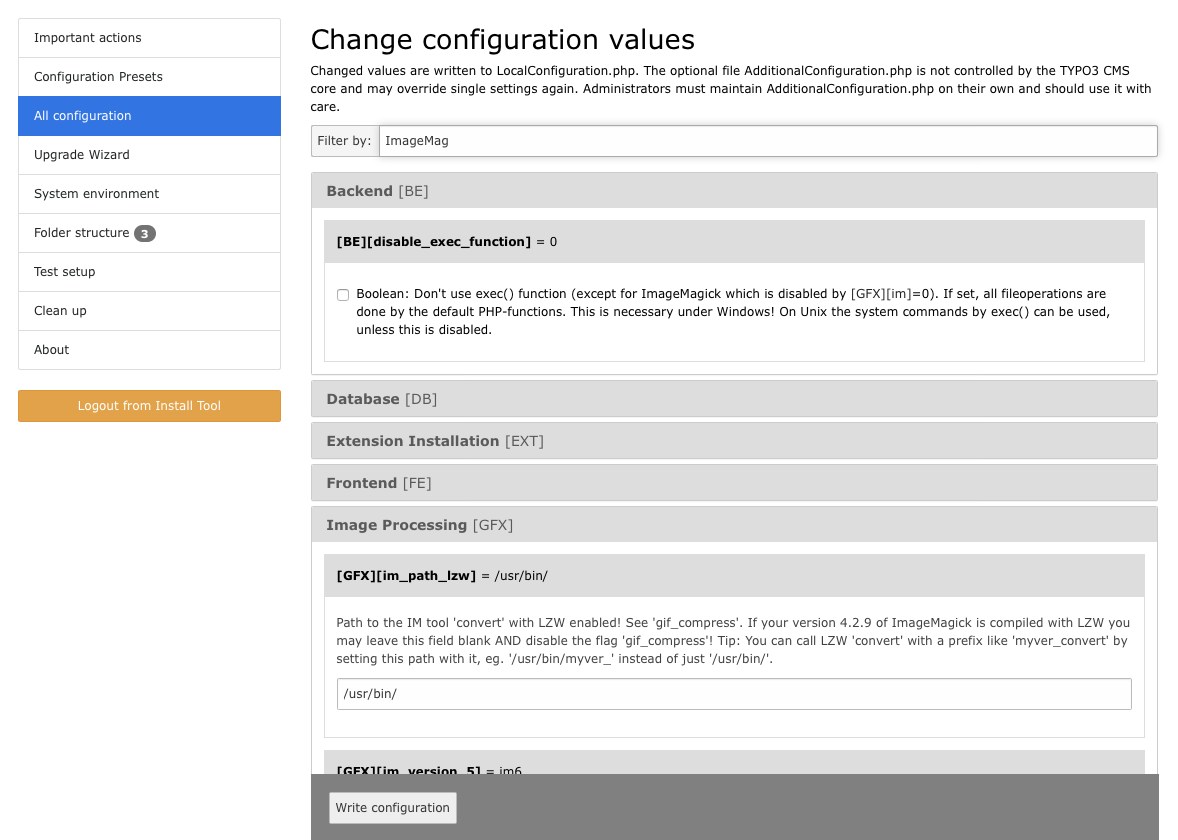
\includegraphics[width=0.7\linewidth]{InDepthChanges/InstallToolBootstrap02.png}
			\end{figure}

	\end{itemize}

\end{frame}

% ------------------------------------------------------------------------------
% LTXE-SLIDE-START
% LTXE-SLIDE-UID:		5216ec9a-f0732d77-ff3b358c-9df3b15a
% LTXE-SLIDE-ORIGIN:	f901074a-4080140f-dd93e505-1e8c2178 English
% LTXE-SLIDE-ORIGIN:	d5acb2d2-159a2d7f-6693f827-30cf1736 German
% LTXE-SLIDE-TITLE:		Form protection API for frontend usage
% LTXE-SLIDE-REFERENCE:	Feature-56633-FormProtectionAPIForFrontEndUsage.rst
% ------------------------------------------------------------------------------

\begin{frame}[fragile]
	\frametitle{In-Depth Changes}
	\framesubtitle{CSRF Protection for Frontend Plugins}

	% decrease font size for code listing
	\lstset{basicstyle=\tiny\ttfamily}

	\begin{itemize}

		\item New class allows usage of the FormProtection API in the frontend

		\item This implements a CSRF protection (Cross-Site Request Forgery)

			\begin{lstlisting}
				$formToken = \TYPO3\CMS\Core\FormProtection\FormProtectionFactory::get()->getFormProtection()->generateToken('news', 'edit', $uid);
				if (
				  $dataHasBeenSubmitted
				  && \TYPO3\CMS\Core\FormProtection\FormProtectionFactory::get()->validateToken(
				    \TYPO3\CMS\Core\Utility\GeneralUtility::_POST('formToken'), 'User setup', 'edit')) {
				  // processes the data
				}
				else {
				  // invalid token!
				}
			\end{lstlisting}

	\end{itemize}

\end{frame}

% ------------------------------------------------------------------------------
% LTXE-SLIDE-START
% LTXE-SLIDE-UID:		b75f64cd-616377a7-286821d4-4a22550b
% LTXE-SLIDE-ORIGIN:	0198b067-68da7843-6a6d3f6d-94cee9b7 English
% LTXE-SLIDE-ORIGIN:	388c7243-b679989c-e2b30dbb-78f1aea4 German
% LTXE-SLIDE-TITLE:		Added LinkBrowser APIs (1)
% LTXE-SLIDE-REFERENCE:	Feature-66369-AddedLinkBrowserAPIs.rst
% ------------------------------------------------------------------------------

\begin{frame}[fragile]
	\frametitle{In-Depth Changes}
	\framesubtitle{Tabs for LinkBrowser (1)}

	% decrease font size for code listing
	\lstset{basicstyle=\tiny\ttfamily}

	\begin{itemize}

		\item This new feature allows to extend the LinkBrowser with new tabs

		\item Each tab is handled by a so called "LinkHandler", which has to implement the
			following Interface:\newline
			\small
				\texttt{\textbackslash TYPO3\textbackslash CMS\textbackslash Recordlist\textbackslash LinkHandler\textbackslash LinkHandlerInterface}
			\normalsize

		\item LinkHandlers are registered in PageTSconfig as follows:

			\begin{lstlisting}
				file {
				  handler = TYPO3\\CMS\\Recordlist\\LinkHandler\\FileLinkHandler
				  label = LLL:EXT:lang/locallang_browse_links.xlf:file
				  displayAfter = page
				  scanAfter = page
				  configuration {
				    customConfig = passed to the handler
				  }
				}
			\end{lstlisting}

	\end{itemize}

\end{frame}

% ------------------------------------------------------------------------------
% LTXE-SLIDE-START
% LTXE-SLIDE-UID:		c4025faf-2da06d69-eb8feb60-37217494
% LTXE-SLIDE-ORIGIN:	7ff322bc-2ace574c-34ddebb5-559fd90c English
% LTXE-SLIDE-ORIGIN:	dfd89b4b-7b4b816c-e5904ba8-2527339b German
% LTXE-SLIDE-TITLE:		Added LinkBrowser APIs (2)
% LTXE-SLIDE-REFERENCE:	Feature-66369-AddedLinkBrowserAPIs.rst
% ------------------------------------------------------------------------------

\begin{frame}[fragile]
	\frametitle{In-Depth Changes}
	\framesubtitle{Tabs for LinkBrowser (2)}

	% decrease font size for code listing
	\lstset{basicstyle=\tiny\ttfamily}

	\begin{itemize}

		\item Options \texttt{displayBefore} and \texttt{displayAfter} define the positions of the tabs

		\item Options \texttt{scanBefore} and \texttt{scanAfter} define the order in which handlers are
			executed when scanning existing links

			\begin{lstlisting}
				$GLOBALS['TYPO3_CONF_VARS']['SC_OPTIONS']['LinkBrowser']['hooks'][1444048118] = [
				  'handler' => \Vendor\Ext\MyClass::class,
				  'before' => [], // optional
				  'after' => [] // optional
				];
			\end{lstlisting}

	\end{itemize}

\end{frame}

% ------------------------------------------------------------------------------
% LTXE-SLIDE-START
% LTXE-SLIDE-UID:		ece63c3e-31418230-aaab20d4-9198523a
% LTXE-SLIDE-ORIGIN:	1ef90646-4f4342dd-3bf0112b-95acba1b English
% LTXE-SLIDE-ORIGIN:	687f24a3-032124a3-7ac41f15-26329962 German
% LTXE-SLIDE-TITLE:		Module Template API (1)
% LTXE-SLIDE-REFERENCE:	Feature-69814-ModuleTemplateAPI.rst
% ------------------------------------------------------------------------------

\begin{frame}[fragile]
	\frametitle{In-Depth Changes}
	\framesubtitle{Module Template API (1)}

	% decrease font size for code listing
	\lstset{basicstyle=\tiny\ttfamily}

	\begin{itemize}

		\item A new Module Template API aims to normalize the implementation of DocHeaders

		\item Example 1: adding a button

			\begin{lstlisting}
				$openInNewWindowButton = $this->moduleTemplate->getDocHeaderComponent()->getButtonBar()
				  ->makeLinkButton()
				  ->setHref('#')
				  ->setTitle($this->getLanguageService()->sL(
				    'LLL:EXT:lang/locallang_core.xlf:labels.openInNewWindow', TRUE
				    ))
				  ->setIcon($this->iconFactory->getIcon('actions-window-open', Icon::SIZE_SMALL))
				  ->setOnClick($aOnClick);

				$this->moduleTemplate->getDocHeaderComponent()->getButtonBar()
				  ->addButton($openInNewWindowButton, ButtonBar::BUTTON_POSITION_RIGHT);
			\end{lstlisting}
	\end{itemize}

\end{frame}

% ------------------------------------------------------------------------------
% LTXE-SLIDE-START
% LTXE-SLIDE-UID:		df7aa091-26a062f7-0d93e138-9844ef73
% LTXE-SLIDE-ORIGIN:	44c8e88e-5668ccb6-3cf424ea-c6a40ecf English
% LTXE-SLIDE-ORIGIN:	1570c8c9-2dfa48e9-058d2d04-bff5465d German
% LTXE-SLIDE-TITLE:		Module Template API (2)
% LTXE-SLIDE-REFERENCE:	Feature-69814-ModuleTemplateAPI.rst
% ------------------------------------------------------------------------------

\begin{frame}[fragile]
	\frametitle{In-Depth Changes}
	\framesubtitle{Module Template API (2)}

	% decrease font size for code listing
	\lstset{basicstyle=\tiny\ttfamily}

	\begin{itemize}
		\item Example 2: adding a menu with menu items

			\begin{lstlisting}
				$languageMenu = $this->moduleTemplate->getDocHeaderComponent()
				  ->getModuleMenuRegistry()->makeMenu()
				  ->setIdentifier('_langSelector')
				  ->setLabel($this->getLanguageService()->sL(
				    'LLL:EXT:lang/locallang_general.xlf:LGL.language', TRUE
				  ));

				$menuItem = $languageMenu->makeMenuItem()
				  ->setTitle($lang['title'] . $newTranslation)
				  ->setHref($href);

				if((int)$lang['uid'] === $currentLanguage) {
				  $menuItem->setActive(TRUE);
				}

				$languageMenu->addMenuItem($menuItem);
				$this->moduleTemplate->getDocHeaderComponent()->getModuleMenuRegistry()->addMenu($languageMenu);
			\end{lstlisting}
	\end{itemize}

\end{frame}


% ------------------------------------------------------------------------------
% LTXE-SLIDE-START
% LTXE-SLIDE-UID:		7d950691-106c1312-73988e58-65579300
% LTXE-SLIDE-ORIGIN:	2ffbc623-117a44dc-923610ec-78a3afc2 English
% LTXE-SLIDE-ORIGIN:	df3ea848-d5406e98-edbd6684-485ff477 German
% LTXE-SLIDE-TITLE:		PSR-7-based Routing for Backend AJAX Requests
% LTXE-SLIDE-REFERENCE:	Feature-69916-PSR-7-basedRoutingForBackendAJAXRequests.rst
% ------------------------------------------------------------------------------

\begin{frame}[fragile]
	\frametitle{In-Depth Changes}
	\framesubtitle{PSR-7 Routing for Backend AJAX Requests}

	% decrease font size for code listing
	\lstset{basicstyle=\tiny\ttfamily}

	\begin{itemize}

		\item To add a route for an AJAX request, file
			\texttt{Configuration/Backend/AjaxRoutes.php}\newline
			can be created with the following content:

			\begin{lstlisting}
				return [
				  // do something
				  'unique_route_name' => [
				    'path' => '/toolcollection/some-action',
				    'target' => \Vendor\Controller\SomeController::class . '::myAction',
				  ]
				];
			\end{lstlisting}

	\end{itemize}

\end{frame}

% ------------------------------------------------------------------------------
% LTXE-SLIDE-START
% LTXE-SLIDE-UID:		138e0e8b-4ad6555c-af94aeff-f080f1ae
% LTXE-SLIDE-ORIGIN:	b68a9d26-30e6d4a0-7bccecf2-ad1f93c6 English
% LTXE-SLIDE-ORIGIN:	cb01cca6-58e91977-d18fa0b3-cba021ab German
% LTXE-SLIDE-TITLE:		Introduced two new Hooks for OpenID (getUserRecord)
% LTXE-SLIDE-REFERENCE:	Feature-44127-HooksForOpenIdToAutomaticallyCreateUserAccounts.rst
% ------------------------------------------------------------------------------
\begin{frame}[fragile]
	\frametitle{In-Depth Changes}
	\framesubtitle{OpenID Hook \texttt{getUserRecord}}

	% decrease font size for code listing
	\lstset{basicstyle=\tiny\ttfamily}

	Two hooks have been added to the OpenID service (1/2)

		\begin{itemize}

			\item Hook 1:\newline
				\smaller\smaller
					\texttt{\$GLOBALS['TYPO3\_CONF\_VARS']['SC\_OPTIONS']['openid']['getUserRecord']}
				\normalsize

				\begin{itemize}
					\item Modifies the user record after it has been fetched, or:
					\item Create a new record if none was found
					\item Parameters \texttt{record}, \texttt{response} and \texttt{authInfo} are passed to the hook
				\end{itemize}

		\end{itemize}

\end{frame}

% ------------------------------------------------------------------------------
% LTXE-SLIDE-START
% LTXE-SLIDE-UID:		ebaa2ec1-cb9ab83c-caf1c997-949504ef
% LTXE-SLIDE-ORIGIN:	b9b259e4-9d35ace7-edff1014-7390d1d1 English
% LTXE-SLIDE-ORIGIN:	ea0bfed8-831666d7-1ba40bb9-7a95723a German
% LTXE-SLIDE-TITLE:		Introduced two new Hooks for OpenID (authRequest)
% LTXE-SLIDE-REFERENCE:	Feature-44127-HooksForOpenIdToAutomaticallyCreateUserAccounts.rst
% ------------------------------------------------------------------------------
\begin{frame}[fragile]
	\frametitle{In-Depth Changes}
	\framesubtitle{OpenID Hook \texttt{authRequest}}

	% decrease font size for code listing
	\lstset{basicstyle=\tiny\ttfamily}

	Two hooks have been added to the OpenID service (2/2)

		\begin{itemize}

			\item Hook 2:\newline
				\smaller\smaller
					\texttt{\$GLOBALS['TYPO3\_CONF\_VARS']['SC\_OPTIONS']['openid']['authRequest']}
				\normalsize

				\begin{itemize}
					\item Modifies the Authentication Request, before it is sent
					\item Can be used to request additional attributes such as a nickname from the OpenID Server for example
					\item Parameters \texttt{authRequest} and \texttt{authInfo} are passed to the hook
				\end{itemize}

		\end{itemize}

\end{frame}

% ------------------------------------------------------------------------------
% LTXE-SLIDE-START
% LTXE-SLIDE-UID:		a01e3464-745b13dd-725fc530-cc98cc96
% LTXE-SLIDE-ORIGIN:	1626edc6-8d93ff84-f64178bf-8e7650df English
% LTXE-SLIDE-ORIGIN:	115a4459-3653bb99-1680d6ab-d8c3c69b German
% LTXE-SLIDE-TITLE:		Hook in BackendUserAuthentication::getDefaultUploadFolder (1)
% LTXE-SLIDE-REFERENCE:	Feature-68895-IntroducedHookInBackendUserAuthenticationgetDefaultUploadFolder.rst
% ------------------------------------------------------------------------------
\begin{frame}[fragile]
	\frametitle{In-Depth Changes}
	\framesubtitle{Hooks and Signals (1)}

	% decrease font size for code listing
	\lstset{basicstyle=\tiny\ttfamily}

	\begin{itemize}

		\item It is now possible to change the upload folder returned by
			\texttt{BackendUserAuthentication::getDefaultUploadFolder()}

		\item Register the hook in file \texttt{ext\_localconf.php} as follows:

			\begin{lstlisting}
				$GLOBALS['TYPO3_CONF_VARS']['SC_OPTIONS']['t3lib/class.t3lib_userauthgroup.php']
				  ['getDefaultUploadFolder'][] =
				  \Vendor\MyExtension\Hooks\DefaultUploadFolder::class . '->getDefaultUploadFolder';
			\end{lstlisting}

	\end{itemize}

\end{frame}

% ------------------------------------------------------------------------------
% LTXE-SLIDE-START
% LTXE-SLIDE-UID:		ba3c2b80-670a8c28-d925bcef-f5d6d03f
% LTXE-SLIDE-ORIGIN:	9c150d50-ee3ba19b-120ef653-e714135c English
% LTXE-SLIDE-ORIGIN:	d1041967-32814ee3-2172e570-4a6d21bd German
% LTXE-SLIDE-TITLE:		Hook in BackendUserAuthentication::getDefaultUploadFolder (2)
% LTXE-SLIDE-REFERENCE:	Feature-68895-IntroducedHookInBackendUserAuthenticationgetDefaultUploadFolder.rst
% ------------------------------------------------------------------------------
\begin{frame}[fragile]
	\frametitle{In-Depth Changes}
	\framesubtitle{Hooks and Signals (2)}

	% decrease font size for code listing
	\lstset{basicstyle=\tiny\ttfamily}

	\small Example:\normalsize

		\begin{lstlisting}
			<?php
			namespace Vendor\MyExtension\Hooks;
			use TYPO3\CMS\Core\Authentication\BackendUserAuthentication;
			use TYPO3\CMS\Core\Resource\Folder;

			/**
			 * Class DefaultUploadFolder
			 */
			class DefaultUploadFolder {

			  /**
			   * Get default upload folder
			   * If there is a folder present with the same name as the last part of the table name use that folder.
			   * @param array $params
			   * @param BackendUserAuthentication $backendUserAuthentication
			   * @return Folder
			   */
			   public function getDefaultUploadFolder($params, BackendUserAuthentication $backendUserAuthentication) {
			    [...]
		\end{lstlisting}

\end{frame}

% ------------------------------------------------------------------------------
% LTXE-SLIDE-START
% LTXE-SLIDE-UID:		b7e36c54-b304c9e6-155b4723-58e38e87
% LTXE-SLIDE-ORIGIN:	a4d7bec0-6c19d8b2-6a6be951-5d5aa0c0 English
% LTXE-SLIDE-ORIGIN:	2f855107-2262065c-c865f953-91b4f0ea German
% LTXE-SLIDE-TITLE:		Hook in BackendUserAuthentication::getDefaultUploadFolder (3)
% LTXE-SLIDE-REFERENCE:	Feature-68895-IntroducedHookInBackendUserAuthenticationgetDefaultUploadFolder.rst
% ------------------------------------------------------------------------------
\begin{frame}[fragile]
	\frametitle{In-Depth Changes}
	\framesubtitle{Hooks and Signals (3)}

	% decrease font size for code listing
	\lstset{basicstyle=\tiny\ttfamily}

	\small Example (continued):\normalsize

		\begin{lstlisting}
			    [...]

			    /** @var Folder $uploadFolder */
			    $uploadFolder = $params['uploadFolder'];
			    $pid = $params['pid'];
			    $table = $params['table'];
			    $field = $params['field'];

			    $matches = [];
			    if (!empty($uploadFolder) && preg_match('/_([a-z]+)$/', $table, $matches)) {
			      $folderName = $matches[1];
			      if ($uploadFolder->hasFolder($folderName)) {
			        $uploadFolder = $uploadFolder->getSubfolder($folderName);
			      }
			    }
			    return $uploadFolder;
			  }
			}
		\end{lstlisting}

\end{frame}

% ------------------------------------------------------------------------------
% LTXE-SLIDE-START
% LTXE-SLIDE-UID:		ee05ac37-4b3912b3-b27c90a1-4f2b8bed
% LTXE-SLIDE-ORIGIN:	2c656d9e-38b9be7a-d590cb6e-21eccd4d English
% LTXE-SLIDE-ORIGIN:	cd6ba83d-9f068dee-b8887ffa-4a2eff29 German
% LTXE-SLIDE-TITLE:		Diverse Änderungen
% LTXE-SLIDE-REFERENCE:	Deprecation-69822-DeprecateSelectFieldTca.rst
% ------------------------------------------------------------------------------
\begin{frame}[fragile]
	\frametitle{In-Depth Changes}
	\framesubtitle{Miscellaneous}

	\begin{itemize}

		\item Using the TCA field type \texttt{select} requires to specify an option \texttt{renderType}

		\item Valid values are:

			\begin{lstlisting}
				'renderType' => 'selectMultipleSideBySide',
				'renderType' => 'selectCheckBox',
				'renderType' => 'selectSingle',
				'renderType' => 'selectSingleBox',
				'renderType' => 'selectTree',
			\end{lstlisting}

	\end{itemize}

\end{frame}

% ------------------------------------------------------------------------------
